\chapter{Jacobi Algorithm}\label{chap:jacobi_algorithm}

The Jacobi algorithm for eigenvalues are first published by Jacobi in 1846~\cite{Jacobi-original-paper-1846} and became widely used in the 1950s after the computer is invented. In this chapter, we will first derive the Jacobi algorithm and discuss its linear convergence. Then the rest of this chapter will focus on two different Jacobi algorithms: Classical and Cyclic-by-row. MATLAB implementation and testing will be given.


\section{Derivation and Convergence}\label{sec:Deriv and Conver}

Given a symmetric matrix $A\in \R\nn$, the idea of the Jacobi algorithm is that at the $k$th step, we use $A^{(k+1)} = Q_{k}\tp A^{(k)}Q_{k}$ to replace $A\iter{k}$, where $Q_{k}$ is orthogonal. We aim to have the property that the off-diagonal entries of $A^{(k+1)}$ are smaller than the off-diagonal entries of $A^{(k)}$. To do this, we use the Givens rotation matrix defined in section~\ref{sec:givens-rotation}.

\begin{definition}
  [$\off$ operator]
  We define the quantity
  \begin{equation}\notag
      \off(A) \coloneqq \sqrt{\|A\|^2_F - \sum_{i=1}^n a^2_{ii}} = \sqrt{\sum_{i=1}^n \sum_{\substack{\text{$j=1$}\\\text{$j\neq i$}}}^n a^2_{ij}},
  \end{equation}
  which is the Frobenius norm of the off-diagonal elements.
\end{definition}

The aim of the Jacobi algorithm on $A$ can be translated to reduce the quantity $\off(A)$. This can be done in 2 steps. 
\begin{enumerate}
  \item Choosing a pair of index $(p,q)$. We assume that $1\leq p < q\leq n$.
  \item Overwriting $A$ by applying $G(p,q,\theta)$ on the matrix $A$ in the way of $$A' = G(p,q,\theta)\tp AG(p,q,\theta),$$ where $\theta$ is chosen such that $A'_{pq}= A'_{qp} = 0$.
\end{enumerate}
Using the Jacobi algorithm on $A$, we produce a sequence of matrices $\big\{A^{(k)}\big\}_{k=0}^\infty$, where 
\begin{equation}\notag
  \begin{cases}
      A^{(0)} = A,  \\
      A^{(k)} = G_{k-1}(p,q,\theta)\tp A^{(k-1)}G_{k-1}(p,q,\theta), & \text{for $k = 1,2,\dots$.}
  \end{cases}
\end{equation}

This set of iterations satisfy

\begin{equation}
  \label{eq:jaco-condition}
  \lim_{k\to\infty}\off(A^{(k)}) = 0.
\end{equation}

In the rest of this section, we will discuss how we can achieve \eqref{eq:jaco-condition} using step 2 and how we can construct such a matrix $G(p,q,\theta)$ given the choice $(p,q)$. Then in the next two sections, we present two different methods of choosing the index $(p,q)$
\begin{itemize}
  \item The Classical Jacobi Algorithm.
  \item The Cyclic-by-row Jacobi Algorithm.
\end{itemize}

Considering the subproblem which only involves four entries of $A$.
\begin{equation}
    \label{eq:2.2}
    \begin{aligned}
        \begin{bmatrix}
            b_{pp} & b_{pq} \\ b_{qp} & b_{qq}
        \end{bmatrix} &= 
        \begin{bmatrix}
            c & s \\ -s & c
        \end{bmatrix}\tp 
        \begin{bmatrix}
            a_{pp} & a_{pq} \\ a_{qp} & a_{qq}
        \end{bmatrix} 
        \begin{bmatrix}
            c & s \\ -s & c
        \end{bmatrix}\\
        & = 
        \begin{bmatrix}
            c^2a_{pp} - cs a_{qp} - cs a_{pq} + s^2a_{qq} &
            cs a_{pp} - s^2 a_{qp} + c^2 a_{pq} - csa_{qq}\\
            c^2a_{pq} + csa_{pp} - csa_{qq} - s^2 a_{pq} &
            csa_{qp} + s^2 a_{pp} + c^2 a_{qq} + csa_{pq}
        \end{bmatrix}.
    \end{aligned}
\end{equation}

Since $A$ is symmetric (symmetry is preserved by orthogonal transformations), we have $a_{pq} = a_{qp}$. Hence we can make further simplification to \eref{eq:2.2}
\begin{equation}
    \label{eq:2.3}
    \begin{bmatrix}
        b_{pp} & b_{pq} \\ b_{qp} & b_{qq}
    \end{bmatrix} =
    \begin{bmatrix}
        c^2 a_{pp} + s^2 a_{qq} -2csa_{pq} & cs(a_{pp} - a_{qq}) + (c^2 -s^2)a_{pq}\\
        cs(a_{pp}-a_{qq}) + (c^2 -s^2)a_{pq} & s^2 a_{pp} + c^2a_{qq} + 2csa_{pq}
    \end{bmatrix}.
\end{equation}
To achieve step 2, we require $b_{pq} = b_{qp} = 0$, which means
\begin{equation}\label{eq:2.4}
    cs(a_{pp}-a_{qq}) + (c^2 -s^2)a_{pq} = 0.
\end{equation}
This equality is essential for us to find the desired Givens rotation and the construction will be discussed in section~\ref{sec:2.3}.

If we take the Frobenius norm on the first line of \eref{eq:2.2} and set $b_{pq}=b_{qp} = 0$, since the Frobenius norm is orthogonally invariant norm (Theorem~\ref{thm:matrix-invariant-norm}), we have 
\begin{equation}\label{eq:2.8}
    b_{pp}^2 + b_{qq}^2 = a_{pp}^2 + a_{qq}^2 + 2a_{pq}^2.
\end{equation}

Using the notations in proposition~\ref{prop:1.3} and the condition $b_{pq} = b_{qp}=0$, we have 
\begin{equation}
    \label{eq:2.5}
    \begin{aligned}
        \off(B)^2 &= \|B\|_F^2 - \sum_{i=1}^n b^2_{ii} = \|A\|_F^2 - \sum_{\substack{i=1\\i\neq p,q}}\big(b^2_{ii}\big) - \big(b^2_{pp} + b^2_{qq}\big)\\
        & = \|A\|_F^2 - \sum^n_{\substack{i=1\\i\neq p,q}}(b^2_{ii}) - a_{pp}^2 - a_{qq}^2 - 2a_{pq}^2 \quad \text{Using \eref{eq:2.8}}\\
        & = \|A\|_F^2 - \sum^n_{\substack{i=1\\i\neq p,q}}(a^2_{ii}) - a_{pp}^2 - a_{qq}^2 - 2a_{pq}^2 \quad \text{By Proposition~\ref{prop:1.3}}\\
        & = \|A\|_F^2 - \sum_{i=1}^n(a^2_{ii}) - 2a_{pq}^2 = \off(A)^2 -2a_{pq}^2.
    \end{aligned}
\end{equation}

Therefore, after $k$ steps and for some choices of the index pair $(p,q)$, we always have 
\begin{equation}\notag
  \off(A\iter{k+1}) = \off(A\iter{k}) - 2a_{pq}^2,
\end{equation}
and this reduction will never terminate until all the off-diagonal entries are zero. However, since each time we introduced a zero, the previous entry we chose will not necessarily remain zero, hence the $\off(A\iter{k})$ will require an infinite number of iterations to converge to zero. In Section~\ref{sec:classical-jacobi}, we proved that even if we choose the largest $a_{pq}$ at each iteration, we still require infinite iteration for $\off(A\iter{k})$ converges to zero.

\subsection{Choices of Givens rotation matrix}\label{sec:2.3}

In this section, we provide a theory to choose $c$ and $s$ for constructing the Givens rotation matrix we need at each iteration. Firstly, if $a_{pq}=0$, there is no need to do further work since $\off(B) = \off(A)$ and we can simply choose $c = 1$ and $s = 0$ which lead to an identity matrix. Otherwise, we look at \eref{eq:2.4}
\begin{equation}
  \label{eq:sec:3.1.1_equality}
    cs(a_{pp}-a_{qq}) + (c^2 -s^2)a_{pq} = 0. \tag{3.6}
\end{equation}
Notice that $c = \cos(\theta)$ and $s = \sin(\theta)$, we have 
\begin{equation}\notag
    \label{2.9}
    \cot(2\theta) = \frac{\cos^2(\theta) - \sin^2(\theta)}{2\cos(\theta)\sin(\theta)} = \frac{c^2 - s^2 }{2cs} = \frac{a_{qq}-a_{pp}}{2a_{pq}} =:\tau.
\end{equation}
By define $t = s/c$, we have transformed \eref{eq:sec:3.1.1_equality} into 
\begin{equation}\label{eq:2.10}
    t^2 + 2\tau t - 1 = 0.
\end{equation}

This quadratic equation can be solved and we would like to choose the root of smaller magnitude.
\begin{equation}\notag
    t_{1,2} = -\tau \pm \sqrt{\tau^2 + 1},\quad \to \quad t_{\mathrm{min}} = 
    \begin{cases}
        -\tau + \sqrt{\tau^2 + 1}, & \ift \tau\geq 0 ; \\
        -\tau - \sqrt{\tau^2 + 1}, & \ift \tau < 0.
    \end{cases}
\end{equation}

Using the fact that $s^2 + c^2 = 1$ and $t_{\mathrm{min}} = s/c$, we can define $c$ and $s$ by 
\begin{equation}\label{eq:2.12}
    s = ct_{\mathrm{min}},\quad c = \frac{1}{\sqrt{1+t_{\mathrm{min}}^2}}.
\end{equation}

Here we choose the smaller roots (in magnitude) of $t$, so that we ensure $\max(t_{\mathrm{min}}) = 1$ (shown in Figure~\ref{fig:1}), hence the angle of rotation is bounded $|\theta|\leq \pi/4$ and this choice turns out to be important for the quadratic convergence as discussed by Sch{\"o}nhage~\ycite[1961]{1961-first-quadratic-convergence-Schu}.
\begin{figure}[ht]
    \centering
    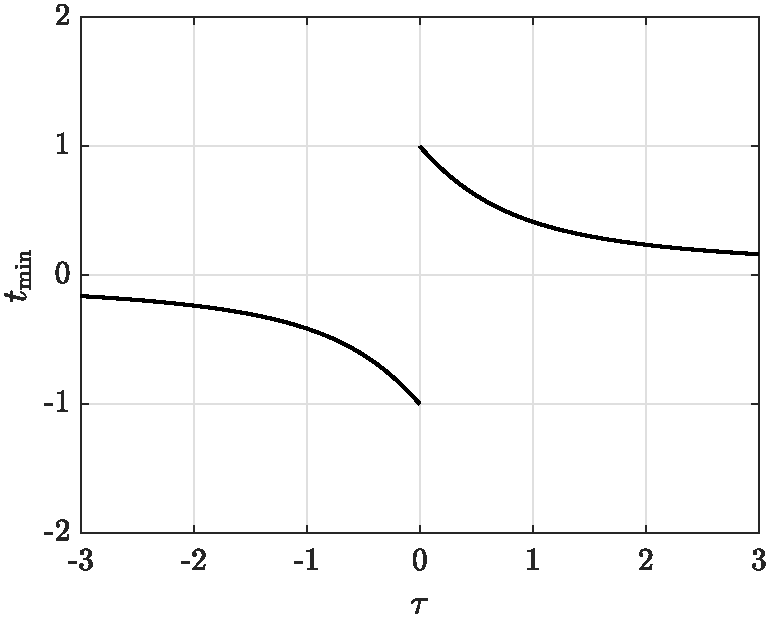
\includegraphics[width=0.5\textwidth]{figs/tmin.pdf}
    \caption{Behavior of the solution $t_{\min}$ of \eqref{eq:2.10}.}
    \label{fig:1}
\end{figure}

\subsection{Implementation and Testing}
Section~\ref{sec:2.3} can be summarized in the following algorithm.
\begin{algorithm}[ht]
    \caption{Given a symmetric matrix $A\in \R\nn$ and integers $p,q$ such that $1\leq p < q\leq n$. This algorithm computes a pair $(c,s)$ to construct $G(p,q,\theta)$ as presented in \eqref{eq:givens}, such that if $B = G(p,q,\theta)\tp A G(p,q,\theta)$, then $b_{pq} = b_{qp} = 0$.}
    \label{alg:jacobi-pair}
    \begin{algorithmic}[1]
        \If {$a_{pq} = 0$}
            \State $c=1,s=0$
        \Else 
            \State $\tau = (a_{qq} - a_{pp})/2a_{pq}$
            \If{$\tau\geq 0$}
                \State $t=-\tau + \sqrt{\tau^2 +1}$
            \Else
                \State $t = -\tau - \sqrt{\tau^2 +1}$
            \EndIf
            \State $c = 1/\sqrt{1+t^2}, s = ct$
        \EndIf
    \end{algorithmic}
\end{algorithm}

When we do the MATLAB implementation, we need to make a minor change to lines 6 and 8. In practice, we need to change these to 
\begin{equation}
  \label{eq:jacobi-pair-preferable-way}
  t = \frac{1}{\tau  \pm  \sqrt{1 + \tau^2}},
\end{equation}
where we choose the positive sign if $\tau \geq 0$ and the minus sign if $\tau <0$. It is easy to prove these two sets of expressions are the same in exact arithmetic, however, they differ in finite precision (See Appendix~\ref{app:algorithm-jacobi-pair}) and \eqref{eq:jacobi-pair-preferable-way} is usually preferable. Then it is straightforward to implement the choice using MATLAB.

\begin{lstlisting}
function [c,s] = jacobi_pair(A,p,q)
if A(p,q) == 0
  c = 1; s = 0;
else
  tau = (A(q,q)-A(p,p))/(2*A(p,q));
  if tau >= 0
    t = 1/(tau + sqrt(1+tau*tau));
  else
    t = 1/(tau - sqrt(1+tau*tau));
  end
  c = 1/sqrt(1+t*t); s = t*c;
end
end
\end{lstlisting}

We can test this function by constructing the matrix $G(p,q,\theta)$ with $(p,q)$ given and examine the $(p,q)$ entry using the following routine,

\begin{lstlisting}
clc; clear; close all;
n = 100; format short e;
A = my_testmatrices(n);
pq = [57,64]; % choose a pair of index
[c,s] = jacobi_pair(A,pq(1),pq(2)); 
% construct the desire Givens rotation matrix
G = eye(n); G([pq(1),pq(2)],[pq(1),pq(2)]) = [c,s;-s,c];
B = G' * A * G;
disp('Before'); disp(A(pq(1),pq(2))); disp(A(pq(2),pq(1)));
disp('After');disp(B(pq(1),pq(2))); disp(B(pq(2),pq(1)));
\end{lstlisting}
This routine should give $b_{pq} = b_{qp} = 0$ where $p = 57$ and $q = 64$.
\begin{lstlisting}
Before
  -9.4140e-01
  -9.4140e-01
After
  -2.2204e-16
  -1.1102e-16
\end{lstlisting}
Before applying the Givens rotations, the entries are $-9.414\times 10^{-1}$ and after such transformation we have $b_{pq}$ and $b_{qp}$ small enough for computers to consider them as zeros. Hence we successfully provide a way of constructing Givens rotations that achieve step 2 as discussed earlier in this section and the remaining part of this chapter is to sophistically choose the index pair $(p,q)$. 

\section{Classical Jacobi Algorithm}\label{sec:classical-jacobi}

From \eref{eq:2.5}, we proved  that $\off(B)^2 = \off(A)^2 - 2a_{pq}^2$, hence it is natural to consider the choice $(p,q)$ such that $a_{pq}^2$ is maximal. This choice was first proposed by Jacobi~\cite{Jacobi-original-paper-1846} in 1846 and the future literature refer to it as the \emph{classical Jacobi algorithm}. We can summarize this choice into Algorithm~\ref{alg:classical Jacobi}.


\begin{algorithm}[ht]
  \caption{({\itshape The classical Jacobi algorithm}) Given a symmetric matrix $A\in\R\nn$ and a positive tolerance $tol$, this algorithm overwrites $A$ with $V\tp AV$ where $V$ is orthogonal.}
  \label{alg:classical Jacobi}
  \begin{algorithmic}[1]
  \State {$V = I_n,\text{ done\_rot = true}$} 
  \While{$\text{done\_rot}$}
    \State $\text{done\_rot = false}$
    \State Choose $(p,q)$ so that $|a_{pq}| = \max_{i\neq j}|a_{ij}|$
    \If{$\abs{a_{pq}} > tol\cdot \norm{A}\sqrt{\abs{a_{pp}a_{qq}}}$}
      \State $\text{done\_rot = true}$
      \State Construct Givens rotation matrix $G$ using Algorithm~\ref{alg:jacobi-pair}
      \State Update $G\tp A G \to A$
      \State Update $VG \to V$
    \Else
      \State Remove the off-diagonal entries of $A$
      \State \textbf{Break}
    \EndIf
  \EndWhile
  \end{algorithmic}
\end{algorithm}

The structure of Algorithm~\ref{alg:classical Jacobi} adapts from~\ycite[2001, Algorithm~2.1]{dht2001} and the stopping criterion is adapted from~\ycite[2013, Section~8.5.5]{van2013mc}, \ycite[2000, Theorem~1.1]{DRMAC2000-preconditioner} and \ycite[1992, Section~1]{demmel92accuracy}.

\subsection{Linear Convergence}

Notice that since $|a_{pq}|$ is chosen to be the largest off-diagonal element, hence we have the inequality
\begin{equation}
    \label{eq:3.1}
    \off(A)^2 \leq N\cdot(2a_{pq}^2),\quad N = \frac{n(n-1)}{2}.
\end{equation}
Using \eref{eq:2.5}, we have 
\begin{equation}
    \label{eq:3.2}
    \begin{aligned}
        \off(B)^2 &= \off(A)^2 - 2a_{pq}^2 \\
        & \leq \off(A)^2 - \frac{1}{N}\off(A)^2 \\
        & = \left(1-\frac{1}{N}\right) \off(A)^2.
    \end{aligned}
\end{equation}

Denote $A^{(k)}$ as the $k$th Jacobi update of $A^{(0)} = A$, then we have the iterative bound 
\begin{equation}
    \label{eq:3.3}
    \off(A^{(k)})^2 \leq \left(1 - \frac{1}{N}\right)^k \off(A^{(0)})^2.
\end{equation}
This implies that the classical Jacobi algorithm converges \emph{linearly} to a diagonal matrix whose entries are the eigenvalues of $A$, and they may appear in any order.

\begin{remark}
    Although the term $\off(A^{(k)})$ decrease at a rate of $(1-1/N)^{1/2}$, if we consider the $N = n(n-1)/2$ steps as one `group' or `sweep' of update, then we actually can expect \emph{asymptotic} quadratic convergence~\ycite[1962]{1962-quadratic-convergence-Jame_Wilkinson} where 
    \begin{equation*}
        \off(A^{(K + 1)})\leq c\cdot \off(A^{(K)})^2, \quad \text{for some }c,
    \end{equation*}
    where $K$ is the number of sweeps.
\end{remark}

\subsection{Implementation and Testing}\label{sec:jacobi-imple-and-testing}

Before we implement the Jacobi algorithm, we need two functions (i) the function that calculates the Frobenius norm of the off-diagonal entries and (ii) the function that finds the index of the maximum entry in modulus.

(i) can be done by carefully selecting the diagonal entries and set to zero, and then calculating the Frobenius norm of the new matrix.
\begin{lstlisting}
function offA = off(A)
n = length(A); % get the dimension of the matrix A
A(1:n+1:n*n) = 0; % set the diagonal entries to zero
offA = norm(A,"fro"); % calculate the norm
end
\end{lstlisting}
The third line of the code will eliminate the diagonal entries, then the fourth line will give us the desired output, $\off(A)$.

(ii) can be implemented using the following function:
\begin{lstlisting}
function [p,q] = maxoff(A)
n = length(A); % dimension of matrix A
A(1:n+1:n*n) = 0; A = abs(A); % clear the diagonal entries
[val, idx1] = max(A);
[~, q] = max(val);
p = idx1(q);
end
\end{lstlisting}

At the fourth line, I use \inline{[val, idx1] = max(A)} to find the index, \inline{idx1}, of the maximum entries of each column and I store the values in \inline{val}. Then we can apply \inline{max()} again to find the index of the maximum entry of \inline{val}, denoted as \inline{q}. Finally, we locate the column number of the maximum entry by calling \inline{idx1(q)} as shown in the sixth line.

Making use of these two functions, we can implement the classical Jacobi algorithm in \mat. The function \inline{jacobi_classical} will take two inputs (i) the symmetric matrix $A^{(0)}\in\R\nn$ and (ii) the tolerance $tol$. I choose to output two matrices, $A$ and $V$ such that $\norm{A\iter{0} V - VA} \lesssim nu_d\norm{A\iter{0}}$ and the number of iterations required. 

Notice that if we would like to update $A^{(k)}$ by $G_k\tp A^{(k)}G_k$, since $A^{(k)},G_k\in\R\nn$, the cost would be $\mathcal O(n^3)$ flops. However, we can utilize proposition~\ref{prop:1.3}, namely, we only need to update the $p$ and $q$th rows and columns of $A^{(k)}$, and this version of the update will only take $O(n)$ flops. We can see this reduction in the following code 

\begin{lstlisting}
[c,s] = jacobi_pair(A,p,q); G = [c s; -s c];
A([p q],:) = G'*A([p q],:); 
A(:,[p q]) = A(:,[p q])*G;
\end{lstlisting}
From the code above, we get both the updated matrix $A^{(k+1)}$ and the orthogonal matrix $G_k$. Line 2 requires a matrix multiplication between $\R^{2\times 2}\times \R^{2\times n}$ which needs $\mathcal O(n)$ flops, and the same argument applies to line 3. Hence when updating the matrix $A^{(k)}$, we only require $\mathcal O(n)$ flops. Assemble all above, we have  

\begin{lstlisting}
function [V,A,counter] = jacobi_classical(A,tol)
counter = 0; n = length(A); V = eye(n); done_rot = true;
tol1 = tol * norm(A);
while done_rot
  if isint(counter/(n*n)), A = (A + A')/2; end % maintain symmetry
  done_rot = false; [p,q] = maxoff(A);
  if abs(A(p,q)) >  tol1 * sqrt(abs(A(p,p) * A(q,q)))
    counter = counter + 1; done_rot = true;
    [c,s] = jacobi_pair(A,p,q);
    J = [c,s;-s,c]; 
    A([p,q],:) = J'*A([p,q],:);
    A(:,[p,q]) = A(:,[p,q]) * J;
    V(:,[p,q]) = V(:,[p,q]) * J;
  else
    A = diag(diag(A)); % output diagonal matrix
    break;
  end
end
end
\end{lstlisting}

After several iterations, although in exact arithmetic, the matrix $A$ should always be symmetric, in floating-point arithmetic, we need to maintain its symmetry as shown in line 5. We can then test our code by the following routine 
\begin{lstlisting}
clc;clear; format short e
n = 1e2; A = randn(n); A = A + A'; tol = 2^(-53);
[V,D,iter] = jacobi_classical(A,tol);
disp('norm(AV - VD)'); disp(norm(A *V - V * D))
\end{lstlisting}

Here we should expect the norm $\norm{AV - VD}$ is about $nu_d \norm{A}$ which is $3.0224\times 10^{-13}$ in our test.

\begin{lstlisting}
norm(AV - VD)
  4.3553e-13
\end{lstlisting}

Hence the algorithm works as expected.

\section{Cyclic-by-row Jacobi Algorithm}\label{sec:cyclic-jacobi}
The classical Jacobi method requires at each step the searching of $n(n-1)$ for one maximum entry in modulus. For $n$ is large, this can be extremely expensive. It will be better if we fixed a sequence of choice $(p,q)$, here in cyclic order shown in the following scheme suggested by~\ycite[1953]{1953-Jacobi-Cyclic-First} and~\ycite[1960, Section~1.2]{forsythe_cyclic_1960}

\begin{equation}\notag
    \begin{aligned}
        (p_0,q_0) &= (1,2), \\
        (p_{k+1},q_{k+1}) & = 
        \begin{cases}
            (p_k,q_{k}+1), & \ift p_k < n-1,q_k < n,\\
            (p_k+1,p_k+2), & \ift p_k < n-1, q_k = n,\\
            (1,2),& \ift p_k = n-1,q_k = n.
        \end{cases}
    \end{aligned}
\end{equation}

We keep using $(p,q)$ in this fashion until we meet the required tolerance and this procedure can be described in Algorithm~\ref{alg:cyclic-jacobi}.

\begin{algorithm}[ht]
  \caption{({\itshape The Cyclic-by-Row Jacobi algorithm}) Given a symmetric matrix $A\in\R\nn$ and a positive tolerance $tol$, this algorithm overwrites $A$ with $V\tp AV$ where $V$ is orthogonal.}
  \label{alg:cyclic-jacobi}
  \begin{algorithmic}
  \State {$V = I_n,\text{ done\_rot = true}$} 
  \While{$\text{done\_rot}$}
    \State $\text{done\_rot = false}$
    \For {$p = 1,\dots, n-1$} 
      \For {$ q = p + 1,\dots, n$}
        \If{$\abs{a_{pq}} > tol\cdot \sqrt{\abs{a_{pp}a_{qq}}}$}
          \State $\text{done\_rot = true}$
          \State Construct Givens rotation matrix $G$ using Algorithm~\ref{alg:jacobi-pair}
          \State Update $G\tp A G \to A$
          \State Update $VG \to V$
        \Else
          \State Remove the off-diagonal entries of $A$
          \State \textbf{Break}
        \EndIf
      \EndFor
    \EndFor
  \EndWhile
  \end{algorithmic}
\end{algorithm}

Similarly, the structure of Algorithm~\ref{alg:cyclic-jacobi} adapts from~\ycite[2001, Algorithm~2.1]{dht2001} and the stopping criterion is adapted from~\ycite[2013, Section~8.5.5]{van2013mc}, \ycite[2000, Theorem~1.1]{DRMAC2000-preconditioner} and \ycite[1992, Section~1]{demmel92accuracy}.

\subsection{Implementation and Testing}
The MATLAB code is similar to the classical Jacobi algorithm, and the only difference is the way of choosing $(p,q)$:

\begin{lstlisting}
function [V,A,iter] = jacobi_cyclic(A,tol,maxiter)
n = length(A); V = eye(n); iter = 0; done_rot = true;
while done_rot && iter < maxiter
  done_rot = false;
  for p = 1:n-1
    for q = p+1:n
      if abs(A(p,q)) > tol * sqrt(abs(A(p,p)*A(q,q)))
        done_rot = true;
        [c,s] = jacobi_pair(A,p,q);
        J = [c,s;-s,c];
        A([p,q],:) = J'*A([p,q],:);
        A(:,[p,q]) = A(:,[p,q]) * J;
        V(:,[p,q]) = V(:,[p,q]) * J;
      end
    end
  end
  if done_rot 
    A = (A + A')/2; iter = iter + 1; 
  else
    A = diag(diag(A));
    return;
  end
end
end
\end{lstlisting}

Notice that, since the cyclic-by-row Jacobi algorithm does not reduce $\off(A\iter{k})$ in the most optimal way, it may require much more iterations than the classical Jacobi algorithm. Hence we restrict the maximum number of iterations by \inline{maxiter} at line 3.

Using the same routine as presented in Section~\ref{sec:jacobi-imple-and-testing}, we have 
\begin{lstlisting}
norm(AV - VD)
   5.9258e-13
\end{lstlisting}
The required tolerance is $nu_d\norm{A} \approx 3.0260\times 10^{-13}$ and therefore we indeed have a eigendecomposition of $A$ at double precision.

\section{Comparision}

In the previous two sections, we discussed both the classical Jacobi algorithm and the cyclic-by-row Jacobi algorithm. However, we need to choose between them. In this section, we will examine the performance concerning both the dimension $n$ and the condition number $\kappa(A)$. We can generate Figure~\ref{fig:classical-cyclic-compare} using code in Appendix~\ref{app:code-for-fig1}. Notice that, in the code, we call a function call \inline{jacobi_eig} and this is the assembled version of the Algorithm~\ref{alg:classical Jacobi} and~\ref{alg:cyclic-jacobi} shown in Appendix~\ref{app:code-full-jacobi}.

\begin{figure}[ht]
\centering
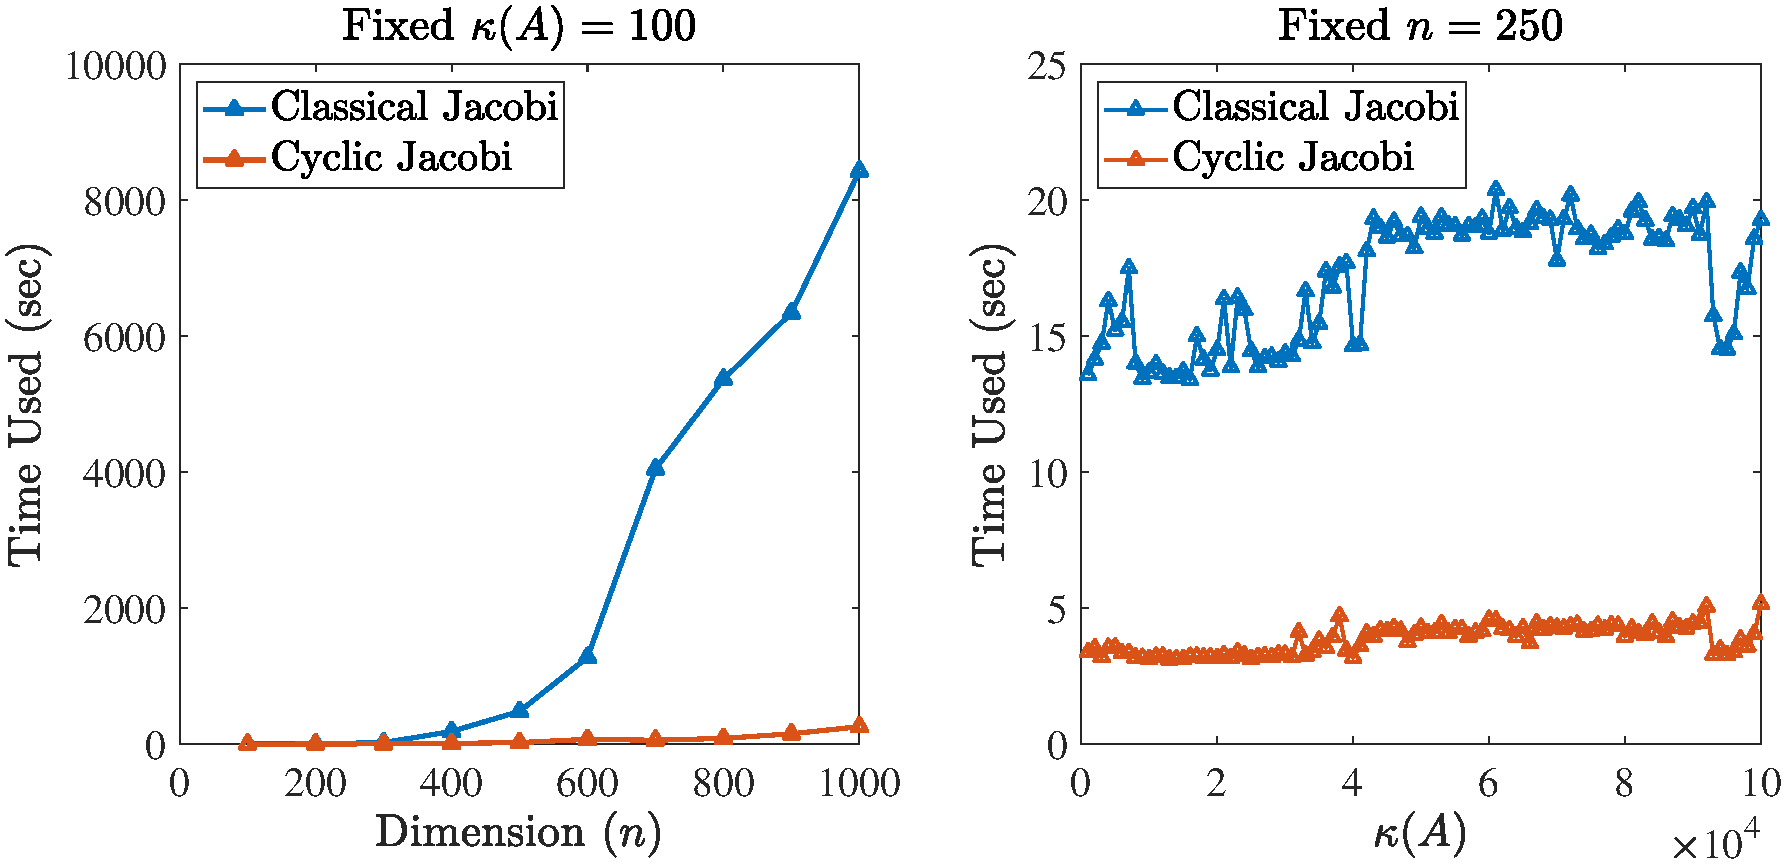
\includegraphics[width=1\textwidth]{figs/classical-cyclic-compare.pdf}
\caption[The time of applying both the classical and the cyclic-by-row Jacobi algorithm on matrix $A\in\R\nn$ with respect to both the dimension $(n)$ and the condition number $\kappa(A)$.]{The time of applying both the codes \inline{jacobi_classical} and \inline{jacobi_cyclic} on a matrix $A\in\R\nn$ with respect to both dimension $(n)$ and the condition number $\kappa(A)$. The left figure fixes the condition number $\kappa(A) = 100$ and the right figure fixes the dimension $n = 250$.}
\label{fig:classical-cyclic-compare}
\end{figure}

From the right figure, we can see the condition number does not affect the time too much. However, from the left figure, we observe that the downside of searching for the maximum off-diagonal entry is significant for large $n$. The cyclic-by-row Jacobi algorithm uses about $1/30$ of the time used by the classical Jacobi algorithm for $n = 1000$. Therefore, although the classical Jacobi reduces the $\off(A)$ in the most optimal way, in practice, we should always stick with the cyclic-by-row Jacobi algorithm.